\documentclass[11pt]{report}

\usepackage{amsmath}
\usepackage{amsfonts}
\usepackage{geometry}
\usepackage{fancyhdr}
\usepackage{mathrsfs}
\usepackage{listings}
\usepackage{xcolor}
\usepackage{graphicx}
\usepackage{wrapfig}
\usepackage{amsthm}
\usepackage{mathrsfs}
\usepackage{textcomp}
\usepackage{float}
\usepackage{setspace}
\usepackage{commath}
\usepackage{amssymb}
\usepackage{indentfirst}
\usepackage{titlesec}
\usepackage{hyperref}

\geometry{left=2.5cm,right=2.5cm,top=2.5cm,bottom=2.5cm}

\setlength{\parindent}{2em}

\pagestyle{fancy}
\lhead{Notes of the Elements of Statistical Learning}                                                
\rhead{Tianyu Wang}  

\title{Notes of the Elements of Statistical Learning}
\author{\href{mailto:wtydbk@hotmail.com}{Tianyu Wang}}
\date{\today}

\theoremstyle{definition}
\newtheorem{defn}{Def}[section]
\newtheorem{exmp}{Ex}[section]

\theoremstyle{plain}
\newtheorem{thm}{Thm}[section]
\newtheorem{lem}[thm]{Lem}
\newtheorem{prop}[thm]{Prop}
\newtheorem*{cor}{Coroll}

\theoremstyle{remark}
\newtheorem*{rem}{Rmk}
\newtheorem*{note}{Note}
\renewcommand{\labelitemi}{$\vcenter{\hbox{\tiny$\bullet$}}$}
%\setlength{\parindent}{0pt}
% \setlength\parindent{0pt}


\begin{document}
\maketitle
\tableofcontents
\newpage
\chapter{Overview of Supervised Learning}

\section{Least Squares and Nearest Neighbors}
Consider two scenario: 
\begin{enumerate}
	\item \textbf{(Better on linear regression)} The training data was generated from bivariate Gaussian distributions with uncorrelated components and different means. 
	\item \textbf{(Better on nearest-neighbor)} The training data came from a mixture of multiple low-variance Gaussian distributions, with individual means themselves distributed as a Gaussian. 
\end{enumerate}
\subsection{Linear Regression Models and Least Squares}
Given $X=(X_1,X_2,...,X_P)$, predict the output $Y$ via model
\begin{equation*}
\hat{Y}=\hat{\beta_0}+\sum_{j=1}^{p}X_j\hat{\beta_j}=X^T\hat{\beta}
\end{equation*}
\begin{itemize}
	\item When $\beta_0=0$, hyperplane $(X,\hat{Y})$ forms a subspace. Otherwise, it is an affine set. 
\end{itemize}

\textbf{Least squares: }$RSS(\beta)=(Y-X\beta)^T(Y-X\beta)=||Y-X\beta||_2^2$
\begin{itemize}
	\item Quatratic$\Rightarrow$Minimum always exists. 
\end{itemize}

\textbf{Unique solution: }$\hat{\beta}=(X^TX)^{-1}X^TY$
\begin{itemize}
	\item Calculated by differentiating $RSS(\beta)$ with respect to $\beta$. 
	\item Minimizing $RSS(\beta)$ $\Leftrightarrow$ choosing $\hat{\beta}$ so that $Y-\hat{Y}$ is orthogonal to the subspace spanned by column vectors of $X$ $\Leftrightarrow$ $\displaystyle\frac{\partial RSS}{\partial\beta}=-2X^T(Y-X\beta)=0$.
	\item \textbf{Do not need a large data set to fit}.  
\end{itemize}

\subsection{Nearest-Neighbor Methods}
Use observations in the training set $\mathcal{T}$ closest to $x$ to form $\hat{Y}$. 
\begin{equation*}
	\hat{Y}(x)=\frac{1}{k}\sum_{x_i\in N_k(x)}y_i
\end{equation*}
\begin{itemize}
	\item Effective number of parameters of kNN is $N/k$ (\href{https://stats.stackexchange.com/questions/357524/why-is-n-k-the-effective-number-of-parameters-in-k-nn}{explanation}). 
	\item Error on train data should be an increasing function of $k$, and equals $0$ for $k=1$. 
	\item Unnecessarily noisy for Gaussian data. 
\end{itemize}
\subsection{From Least Squares to Nearest Neighbors}
\textbf{Linear boundary from least squares}: smooth, relies heavily on the linear assumption. Low variance and high bias. 

\textbf{kNN}: Does not rely on assumptions about underlying data. Any subregion depends on input points and their position. High variance and low bias. 
\begin{itemize}
	\item 1-nearest-neighbor captures a large percentage of the market for low-dimensional problems. 
\end{itemize}

Ways in which these procedures are enhanced
\begin{itemize}
	\item Kernel methods use weights that decrease smoothly to zero with distance from the target method instead of 0/1 in kNN. 
	\item In high dimensional spaces the distance kernels are modified to emphasize some variables more than others. 
	\item Local regression fits linear models by locally weighted least squares rather than fitting constants locally. 
	\item Basis expansion of the inputs to improve complexity of linear model. 
	\item Projection pursuit/NN models: nonlinear transform of linear models
\end{itemize}

\section{Statistical Decision Theory}
\subsection{Quantitative output}
Let $X\in\mathbb{R}^p, Y\in\mathbb{R}$ with joint distribution $Pr(X,Y)$. 

\textbf{Goal}: Find a function $f(X)$ for predicting $Y$, which requires a \textit{loss function} $L(Y, f(X))$. 

\textbf{Squared error loss}: 
\begin{align*}
	L(Y,f(X))=&(Y-f(X))^2\\
	EPE(f)=&E(Y-f(X))^2=\int[y-f(x)]^2Pr(dx,dy)\\
	=&\int[y-f(x)]^2Pr(dy|dx)Pr(dx)=E_XE_{Y|X}([Y-f(X)]^2|X)
\end{align*}
where EPE stands for Expected Prediction Error. I$u(x,t)=0$ when $x<0$ t suffices to minimize EPE pointwise
\begin{equation*}
\end{equation*}
Thus when the measure is squared error, $E(Y|X=x)$ is the best solution. 

~

\textbf{kNN}: 
\begin{equation*}
	\hat{f}(x)=\text{Avg}(y_i|x_i\in N_k(x))
\end{equation*}
\begin{itemize}
	\item Expectation is approximated by averaging
	\item Conditioning at a point is relaxed to a region
	\item As $N,k\rightarrow\infty$ such that $k/N\rightarrow0$, $\hat{f}(x)\rightarrow E(Y|X=x)$
	\begin{itemize}
		\item Since we do not have many samples in most cases, we can usually get a more stable model if some more structured model is appropriate. 
	\end{itemize}
	\item Assumes $f(x)$ is well approximated by a locally constant function. 
\end{itemize}

~

\textbf{Linear Regression}:Let $f(x)=x^T\beta$ and differentiating $E(Y-f(X))^2$, we have optimal $\beta$
\begin{equation*}
	\beta=[E(XX^T)]^{-1}E(XY)
\end{equation*}
The least squares solution just replace the expectation by averages on the training data. 
\begin{itemize}
	\item Assumes $f(x)$ is well approximated by a globally linear function
\end{itemize}

~

If we use $L_1$ loss instead of $L_2$, the solution will becomes the conditional median
\begin{equation*}
	\hat{f}(x)=\text{median}(Y|X=x)
\end{equation*}
\begin{itemize}
	\item A different measure of location
	\item More robust than conditional mean
\end{itemize}

\subsection{Categorical output}
Let the categorical variable be $G$, $K=card(\mathcal{G})$, $K\times K$ matrix $L$ be its loss function, $L_{ii}=0, L_{ij}\ge0$, $L(k,l)$ be the cost of wrong prediction(0/1 in most cases). 
\begin{align*}
	EPE=&E[L(G, \hat{G}(X))]\\
	=&E_X\sum_{k=1}^{K}L[\mathcal{G}_k, \hat{G}(X)]Pr(\mathcal{G}_k|X)\\
	\hat{G}(x)=&argmin_{g\in\mathcal{G}}\sum_{k=1}^{K}L[\mathcal{G}_k, g]Pr(\mathcal{G}_k|X=x)\\
\end{align*}
With 0-1 loss, it can by simplified as
\begin{align*}
	\hat{G}(x)=&argmin_{g\in\mathcal{G}}[1-Pr(g|X=x)]\\
	=&\mathcal{G}_k \text{ if } Pr(\mathcal{G}_k|X=x)=\max_{g\in\mathcal{G}}Pr(g|X=x)	
\end{align*}
It is known as \textit{Bayes classifier}, says we classify the most probable class with conditional distribution $Pr(G|X)$. The error rate here is called \textit{Bayes rate}. 

\section{Local Methods in High Dimensions}
In \textbf{low dimension space}, kNN can always find the theoretically optimal conditional expectaion with a large training set. 
\begin{itemize}
	\item Not work in high dimentional data: \textit{Curse of dimensionality}
\end{itemize}
\begin{exmp}
	Consider $N$ data points uniformly distributed on a unit ball, the median distance from the origin to the closet data point is
	\begin{equation*}
	d(p,N)=(1-\frac{1}{2}^{1/N})^{1/p}
	\end{equation*}
	\begin{itemize}
		\item Let $N=500,p=10\Rightarrow d(p,N)=0.52\Rightarrow$Most points are closer to boundary but not other points$\Rightarrow$Must extrapolate from samples but not interpolate between them. 
		\item Sampling density is proportional to $N^{1/p}$
	\end{itemize}
\end{exmp}
\begin{exmp}
	Consider 1000 $x_i$ from $U([-1,1]^p)$, $Y=f(X)=exp(-8||X||^2)$, then use 1-NN to predict $y_0$ at $x_0=0$, we have \textit{bias-variance decomposition}
	\begin{align*}
		MSE(x_0)=&E[f(x_0)-\hat{y}_0]^2=E[\hat{y}_0-E[\hat{y}_0]]^2+[E[\hat{y}_0]-f(x_0)]^2\\
		=&Var(\hat{y}_0)+Bias^2(\hat{y}_0)
	\end{align*}
	When dimension increase, we will find that distance of the closet point to $0$ increase. The bias will also significantly increase. 
	\begin{itemize}
		\item Complexity of functions of many variables grow exponentially with the dimension--Need exponential growth of the size of the training set to maintain accuracy. 
	\end{itemize}
	If we use function which only cares about a few dimensions like $f(X)=\frac{1}{2}(X_1+1)^3$, the bias will be stable, but the variance will increase a lot. 
\end{exmp}

~

\textbf{Linear model}

Let $Y=X^T\beta+\epsilon,\epsilon\sim N(0,\sigma^2)$, than for test point $x_0$,  $\hat{y}_0=x_0^T\hat{\beta}_0=x_0^T\beta+\sum_{i=1}^Nl_i(x_i)\epsilon_i$, $l_i$ is the $i$th element of $X(X^TX)^{-1}x_0$. Since the model under the least squares is unbiased, we have
\begin{align*}
	EPE(x_0)=&E_{y_0|x_0}E_{\mathcal{T}}(y_0-\hat{y}_0)^2\\
	=&Var(y_0|x_0)+E_{\mathcal{T}}[\hat{y}_0-E_{\mathcal{T}}\hat{y}_0]^2+[E_{\mathcal{T}}\hat{y}_0-x_0^T\beta]^2\\
	=&Var(y_0|x_0)+Var_{\mathcal{T}}(\hat{y}_0)+Bias^2(\hat{y}_0)\\
	=&\sigma^2+E_{\mathcal{T}}x_0^T(X^TX)^{-1}x_0\sigma^2+0^2
\end{align*}
When $N$ is large and $\mathcal{T}$ is selected at random, assume $E[X]=0$, then $X^TX\rightarrow NCov(X)$
\begin{align*}
	E_{x_0}EPE(x_0)\sim&E_{x_0}x_0^TCov(X)^{-1}x_0\sigma^2/N+\sigma^2\\
	=&trace[Cov(X)^{-1}Cov(x_0)]\sigma^2/N+\sigma^2\\
	=&\sigma^2(p/N)
\end{align*}
Thus expected EPE increases as a linear function of $p$ with slope $\sigma^2/N$. 

\section{Statistical Models, Supervised Learning and Function Approximation} 
Goal: find a $\hat{f}(x)$ of $f(x)$. Squared error lead to $f(x)=E(Y|X=x)$, but they may fail
\begin{itemize}
	\item If the dimension is too high, nearest neighbors can not be close to the target and cause large error. 
	\item If the structure is known, this can be used to reduce bias and variance. 
\end{itemize}
\subsection{A Statistical Model for the Joint Distribution $Pr(X,Y)$}
Suppose our data comes from $Y=f(X)+\epsilon$








\chapter{Linear Methods for Regression}
%% TODO LIST
% LAR REGRESSION
% MULTIPLE OUTCOME SHRINKAGE AND SELECTION
% More on the Lasso and Related Path Algorithms

Useful in situations with small numbers of training cases, low signal-to-noise ratio, 
or sparse data. 
\section{Linear Regression Models and Least Squares}
Consider linear model
\begin{equation*}
	f(X)=\beta_0+\sum_{j=1}^{p}X_j\beta_j
\end{equation*}
which assume the regression function $E(Y|X)$ linear or the linear model is a good 
approximation. 
Here $X_j$ can be
\begin{itemize}
	\item Quantitative inputs
	\item Transformation/Basis expansion of inputs e.g. log, square-root, polynomial
	\item Numeric/dummy coding of the levels of the inputs
\end{itemize}
\begin{equation*}
	RSS(\beta)=(y-X\beta)^T(y-X\beta)
\end{equation*}
$X$ has full column rank$\Rightarrow X^TX$ positive definite. 

By solution, we have $\hat{y}=X\beta=X(X^TX)^{-1}X^TY, \hat{y_i}=x_i^T\hat{\beta}$
\begin{itemize}
    \item $H=X(X^TX)^{-1}X^T$: hat matrix, which computes the orthogonal projection 
    from $Y$ to $\hat{Y}$. 
\end{itemize}

When columns of $X$ are not independent
\begin{itemize}
    \item Perfectly correlated$\Rightarrow X^TX$ singular, $\hat{\beta}$ not uniquely 
    defined. However, $\hat{y}$ are still the projection from $y$ to column space of 
    $X$. 
	\begin{itemize}
        \item May appear when number of inputs $p$ exceed the number of training cases $N$, 
        where features reduced by filtering or fitting controlled by regularization. 
	\end{itemize}
\end{itemize}

If $y_i$ are uncorrelated with constant variance $\sigma^2$ and $x_i$ are fixed
(non random), then we have estimation
\begin{align*}
Var(\hat{\beta})=&E[(\hat{\beta}-\beta)(\hat{\beta}-\beta)^T]
=E[((X^TX)^{-1}X^T\epsilon)((X^TX)^{-1}X^T\epsilon)^T]=(X^TX)^{-1}\sigma^2\\
\hat{\sigma}^2=&\frac{1}{N-p-1}\sum\limits_{i=1}^N(y_i-\hat{y_i})^2
\end{align*} 
where $N-p-1$ makes $\hat{\sigma^2}$ is an unbiased estimation because 
$\sum\limits_{i=1}^N(y_i-\hat{y_i})^2\sim \sigma^2\chi^2_{N-p-1}$. 

Now we assume the linearity of the model and deviations of $Y$ around its expectation 
are additive and Gaussian,  consider the model
\begin{equation*}
Y=E(Y|X_1,...,X_p)+\epsilon=\beta_0+\sum\limits_{j=1}^pX_j\beta_j+\epsilon
\end{equation*}
where $\epsilon\sim N(0,\sigma^2)$, 
then $\hat{\beta}\sim N(\beta,(X^TX)^{-1}\sigma^2), 
(N-p-1)\hat{\sigma}^2\sim \sigma^2\chi_{N-p-1}^2$, and $\hat{\beta},\hat{\sigma}^2$ 
statistically independent. 

~

To test \textbf{whether $\beta_j=0$}, we consider Z-score
\begin{equation*}
	z_j=\frac{\hat{\beta}_j}{\hat{\sigma}\sqrt{v_j}}
\end{equation*}
where $v_j$ is the $j$th diagonal element of $(X^TX)^{-1}$, under null hypothesis, 
$z_j$ is distributed as $t_{N-p-1}$, thus a large value of $z_j$ will reject the null 
hypothesis. 
\begin{itemize}
	\item When $\hat{\sigma}$ is replaced by $\sigma$, $z_j$ is normally distributed. 
	\item Difference of tail quantiles will be small when sample size increases. 
\end{itemize}

~

To test the \textbf{significance of groups of coefficients}, e.g. whether a variable 
can be excluded, we need to test whether its coefficients can all be set to zero, 
here we use F-statistics
\begin{equation*}
F=\frac{(RSS_0-RSS_1)/(p_1-p_0)}{RSS_1/(N-p_1-1)}
\end{equation*}
where $RSS_1$ is the residual sum of squares with $p_1+1$ parameters, $RSS_0$ for 
the nested smaller model with $p_0+1$ parameters, having $p_1-p_0$ constrained to 
be $0$, F statistics measures the change in residual sum of squares per additional 
parameter in the bigger model. 

Under Gaussian assumption and null hypothesis that smaller model is correct, 
$F\sim F_{p_1-p_0,N-p_1-1}$. 
\begin{itemize}
	\item $z_j$ is equivalent to F statistics when only drop one coefficient. 
    \item When $N$ is large enough, quantiles of $F_{p_1-p_0,N-p_1-1}$ approach those 
    of the $\chi^2_{p_1-p_0}$
\end{itemize}

When we can isolate $\beta_j$ to obtain a $1-2\alpha$ confidence interval for 
$\beta_j$
\begin{equation*}
    (\hat{\beta}_j-z^{(1-\alpha)}v_j^{\frac{1}{2}}\hat{\sigma}, 
    \hat{\beta}_j+z^{(1-\alpha)}v_j^{\frac{1}{2}}\hat{\sigma})
\end{equation*}
where $z^{(1-\alpha)}$ is the $1-\alpha$ percentile of normal distribution. 

We can also obtain an approximate confidence set for the entire parameter vector 
$\beta$
\begin{equation*}
    C_{\beta}=\{\beta|(\hat{\beta}-\beta)^T(\hat{\beta}-\beta)\le\hat{\sigma}^2 
    {\chi^2_{p+1}}^{(1-\alpha)} \}
\end{equation*}
This confidence set for $\beta$ generates a corresponding confidence set for 
$f(x)=x^T\beta$, namely $\{x^T\beta|\beta\in C_{\beta}\}$

~

Another way of comparing significance between different variables: Use 
Z-score=mean/std of coefficient and compare Z-score of different variables. 
Z-score$>2$ implies significance at 5\% level

\subsection{The Gauss-Markov Theorem}
\begin{itemize}
    \item Least squares estimates of $\beta$ have the smallest variance among all 
    linear unbiased estimates. 
	\item Unbiased estimation may not be a wise choice. 
\end{itemize}

Consider linear combination of parameters $\theta=a^T\beta$, then the least square 
estimates of $a^T\beta$ is
\begin{align*}
	\hat{\theta}=&a^T\hat{\beta}=a^T(X^TX)^{-1}X^TY\\
    E(a^T\hat{\beta})=&E(a^T(X^TX)^{-1}X^Ty)=
    a^T(X^TX)^{-1}X^TE(y)=a^T(X^TX)^{-1}X^TX\beta=a^T\beta
\end{align*}
Thus $a^T\hat{\beta}$ is unbiased if the linear model is correct. 

\begin{thm}
    (Gauss-Markov theorem) If we have any other unbiased linear estimator 
    $\tilde{\theta}=c^Ty$ for $a^T\beta$, then $Var(a^T\hat{\beta})\le Var(c^Ty)$
\end{thm}
\begin{proof}
	Triangle inequality. 
\end{proof}
\begin{rem}
	Can be extended to entire parameter $\beta$ with a few more definition. 
\end{rem}

Now consider 
\begin{equation*}
    MSE(\tilde{\theta})=E(\tilde{\theta}-\theta)^2=
    Var(\tilde{\theta})+[E(\tilde{\theta})-\theta]^2
\end{equation*}
There may exist estimators with little bias and huge reduction on variance, 
which brings them less MSE. Recall that for $Y_0=f(x_0)+\epsilon_0,
\tilde{f}(x_0)=x_0\tilde{\beta}$, 
\begin{equation*}
    E(Y_0-\tilde{f}(x_0))^2=\sigma^2+E(x_0^T\tilde{\beta}-f(x_0))^2
    =\sigma^2+MSE(\tilde{f}(x_0))
\end{equation*}
We have prediction error is related to MSE. 

\subsection{Multiple Regression from Simple Univariate Regression}
Consider univariate model $Y=X\beta+\epsilon$. Then we have
\begin{align*}
\hat{\beta}=\frac{<x,y>}{<x,x>},\quad r=t-x\hat{\beta}
\end{align*}
We can generate a similar model for a $p$-variable model. 

By Schmidt orthogonalization, we can generate an orthogonal basis for the column space, 
and
\begin{equation*}
\hat{\beta}_p=\frac{<z_p,y>}{<z_p,z_p>}
\end{equation*}
It is actually the regression coefficient of $y$ on $x_p$. We can also see that $j$th
coefficient is the residual after regressing $x_j$ on $x_0,x_1,...,x_{j-1},x_{j+1},...x_p$. 

If $x_p$ is highly correlated to some other $x_k$'s, residual vector $z_p$ should be
close to 0, and $\hat{\beta}_p$ would be very unstable. 
\begin{equation*}
Var(\hat{\beta}_p)=\frac{\sigma^2}{<z_p,z_p>}
\end{equation*}
It means the precision with which we can estimates $\hat{\beta}_p$ depends on how much
of $x_p$ can be explained by other $x_k$'s. 

We may also apply $QR$ decomposition on $X=QR$, where $Q$ is an $N\times (p+1)$ 
orthogonal matrix, $Q^TQ=I$, $R$ is a $(p+1)\times (p+1)$ upper triangular matrix. 
Then the solution is given by
\begin{align*}
\hat{\beta}=R^{-1}Q^Ty,\quad \hat{y}=QQ^Ty
\end{align*}

\subsection{Multiple Outputs}
Suppose we want to predict $Y_1,...,Y_k$ with $ X_0,X_1,...X_p $, we assume a linear model
\begin{align*}
Y_k=&\beta_{0k}+\sum_{j=1}^pX_j\beta_{jk}+\epsilon_k=f_k(X)+\epsilon_k\\
Y=&XB+E\\
RSS(B)=&tr[(Y-XB)^T(Y-XB)]\\
\hat{B}=&(X^TX)^{-1}X^TY
\end{align*}
Hence the coefficients for $Y_k$ does not depend on other variable's least square estimation. 

If $Cov(\epsilon)=\Sigma$, we have
\begin{equation*}
RSS(B;\Sigma)=\sum_{i=1}^N(y_i-f(x_i))^T\Sigma^{-1}(y_i-f(x_i))
\end{equation*}
It arises naturally from Gaussian. If $\Sigma_i$ vary from observation, then 
$\hat{B}=(X^TX)^{-1}X^TY$ is no longer the case. 

\section{Subset Selection}
Why we are always not satisfied with OLS estimation
\begin{itemize}
\item \textit{Low bias but large variance}. Can be improved by shrinking/setting some coefficients
to zero, which sacrifice a little bit of bias but reduce the variance. 
\item \textit{Interpretion}. We want to get a smaller subset that exhibit the strongest
effects from many predictors. AKA sacrifice small details to get the "big picture". 
\end{itemize}
Subset selection is a discrete process and may still have high variance, so doesn't
reduce the prediction error of the full model. 
\subsection{Best-Subset Selection}
Find each $k\in\{0,1,2,...p\}$, the subset of size $k$ gives smallest RSS. Note that
RSS is always a decreasing function of $k$, which makes it cannot be used to choose
$k$. Choosing $k$ is about the trade-off between bias and variance. Typically we use 
the smallest model that minimizes an estimate of the expected prediction error. 
\subsection{Forward- and Backward-Stepwise Selection}
Here we try to find a good path through subsets but not search all of them. 

\textbf{Forward-stepwise selection}: Starts with the intercept, then adds the 
predictor that most improves the fit. Methods like QR decomposition an make this 
fast. 
\begin{itemize}
\item Can always be used
\item It is a greedy approach, which might be sub-optimal. 
\item However, it is computational, and has lower covariance(perhaps higher bias). 
\end{itemize}

\textbf{Backward-stepwise selection}: Starts with the whole model, then deletes the 
predictor that least impacts the fit(variable with lowest Z-score). 
\begin{itemize}
\item Only used when $N>p$. 
\item Similar performance 
\end{itemize}

Some packages can do both at the same time. Criterion like AIC could be a good idea, 
which takes proper account of the number of parameters. Add or drop will be performed
that minimizes the AIC. On the other hand, F-statistics is kind of out of fashion. 

\subsubsection{Forward-Stagewise Regression}
Slow and inefficient, but may pay dividends in high-dimensional problems. 

\section{Shrinkage Methods}
More continuous compared with subset selection, doesn't suffer as much from high
variability. 
\subsection{Ridge Regression}
\begin{equation*}
\hat{\beta}^{\text{ridge}}=
argmin_{\beta}\left\{||y-X\beta||_2^2+\lambda ||\beta||_2^2\right\}
\end{equation*}
Idea of penalizing parameters is also used in neural network as \textit{weight
decay}. 

The problem is equivalent to
\begin{align*}
\hat{\beta}^{\text{ridge}}=&
argmin_{\beta}\left\{||y-X\beta||_2^2\right\} \text{ subject to }||\beta||_2^2<t
\end{align*}
where $t$ and $\lambda$ have one-to-one correspondence. 
When there are correlated variables, there may be mildly large and small parameters, 
Imposing a size constraint can solve this problem. 

The solution is
\begin{equation*}
\hat{\beta}^{\text{ridge}}=(X^TX+\lambda I)^{-1}X^Ty
\end{equation*}
$\lambda I$ makes the problem always nonsingular even if $X^TX$ is singular. 

In the case of orthonormal inputs, Ridge is just a scaled OLS estimates 
$\hat{\beta}^{\text{ridge}}=\hat{\beta}/(1+\lambda)$. 

\textbf{SVD insight}
Consider SVD $X=UDV^T$, here $U$ span the column space of $X$, $V$ span the row 
space, $d_1\ge d_2\ge...\ge d_p\ge0$. When there is $d_j=0$, $X$ is singular. 
$U$ and $Q$(in QR decomposition) are generally different orthogonal bases for 
the column space of $X$. 

With SVD, we have $X\hat{\beta}^{\text{ls}}=UU^Ty$, and ridge solution
\begin{equation*}
X\hat{\beta}^{\text{ridge}}=\sum_{j=1}^p u_j\frac{d_j^2}{d_j^2+\lambda}u_j^Ty
\end{equation*}

It shows Ridge shrinks the coordinates by $d_j^2/(d_j^2+\lambda)$. It shows 
greater amount is shrinked for small $d_j^2$. Note that $X^T=VD^2V^T$. $v_j$ the 
PC directions of $X$. $z_1=Xv_1=u_1d_1$ explains the most variance, and 
$Var(z_1)=d_1^2/N$. $z_1$ the first PC of $X$. 

$\displaystyle \sum_{j=1}^p\frac{d_j^2}{d_j^2+\lambda}$: \textit{Effective 
degrees of freedom}

\subsection{Lasso Regression}
\begin{align*}
    \hat{\beta}^{\text{lasso}}=&
    argmin_{\beta}\left\{||y-X\beta||_2^2\right\} \text{ subject to }
    ||\beta||_1<t\\
    =&argmin_{\beta}\left\{||y-X\beta||_2^2+\lambda ||\beta||_1\right\}
\end{align*}
Does a kind of continuous subset selection. 
$\hat{\beta}^{\text{lasso}}_j=sign(\hat{\beta}_j)(\abs{\hat{\beta_j}}-\lambda)_+$
\subsection{Discussion: Subset Selection, Ridge Regression and the Lasso}
Actually, $\hat{\beta}^{\text{bestSubset}}_j=\hat{\beta}_j\cdot
I(\abs{\hat{\beta}_j}\ge \hat{\beta}_{(M)})$
\begin{equation*}
    \hat{\beta}^{\text{bestSubset}}=
    =argmin_{\beta}\left\{||y-X\beta||_2^2+\lambda \sum_j\abs{\beta_j}^0\right\}
\end{equation*}
$\lambda \sum_j\abs{\beta_j}^0$: counts of nonzero values. 

Elastic-penalty: 
\begin{equation*}
\lambda\sum_{j=1}^p(\alpha\beta_j^2+(1-\alpha)\abs{\beta_j})
\end{equation*}
It is a compromise between ridge and lasso: selects variables like lasso, and 
shrinks together the coefficient of correlated predictors like ridge. Has
computational advantages over $L_q$ penalties. 

\subsection{Least Angle Regression(LAR)}
A "democratic" version of forward stepwise regression. Extremely efficient. 
\begin{figure}[H]
    \centering
    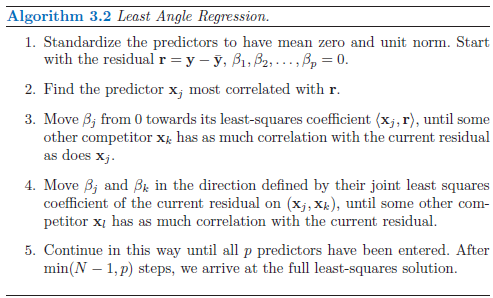
\includegraphics[width=0.7\textwidth]{Figures/LARAlgo}
\end{figure}
Let $\mathcal{A}_k$ be the active set at step $k$, $\beta_{\mathcal{A}_k}$ be the 
coefficient vector. There will be $k-1$ nonzero values and one zero. Let 
$r_k=y-X_{\mathcal{A}_k}\beta_{\mathcal{A}_k}$, then the direction for this step is
\begin{equation*}
\delta_k=(X_{\mathcal{A}_k}^TX_{\mathcal{A}_k})X_{\mathcal{A}_k}^Tr_k
\end{equation*}
Then coefficient profile evolves as
$\beta_{\mathcal{A}_k}(\alpha)=\beta_{\mathcal{A}_k}+\alpha\cdot \delta_k$. 
Let $u_k=X_{\mathcal{A}_k}\delta_k$, it makes the smallest and equal angle with each 
predictor in $\mathcal{A}_k$.  With LAR, we can know the step length at the beginning
of each step. 

%TODO:

\section{Methods of Derived Input Directions}
Large number of inputs with high correlation. This section describes how to linearly
combine $X_j$ to $Z_m$ used in regression. 
\subsection{Principal Components Regression}
Since $Z_m$ here are orthogonal, when regress $y$ for some $M<p$,
\begin{equation*}
\hat{y}_{(M)}^{\text{per}}=\bar{y}1+\sum_{m=1}^M\hat{\theta}_mz_m,\quad
\hat{\theta}_m=\frac{<z_m,y>}{<z_m,z_m>}
\end{equation*}
Since $z_m=Xv_m$, we have
\begin{equation*}
\hat{\beta}^{\text{per}}(M)=\sum_{m=1}^M\hat{\theta}_mv_m
\end{equation*}
Compared with Ridge, it discards the $p-M$ smallest eigenvalue components. 
 
\subsection{Partial Least Squares}
Assume $x_j$ is normalized(PLS and principal components regression are not
scale invariant). It begins by
\begin{equation*}
\hat{\varphi}_{1j}=<x_j,y>, \quad z_1=\sum_j\hat{\varphi}_{1j}x_j
\end{equation*}
Hence in the construction, inputs are weighted by the strength of their univariate 
effect on $y$. 
\begin{figure}[H]
    \centering
    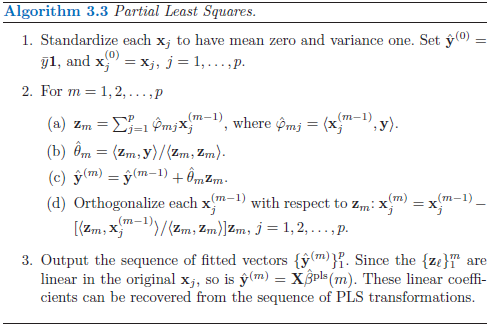
\includegraphics[width=0.7\textwidth]{Figures/PLSAlgo}
    \label{fig:}
\end{figure}
PLS seeks directions that have high variance and high correlation with the response. 
In particular, the $m$th principal component direction $v_m$ solves
\begin{equation*}
\max_\alpha Var(X\alpha) \quad\text{ subject to } 
||\alpha||=1,~\alpha^TSv_l=0,~l=1,2,...,m-1
\end{equation*}
where $S$ is the covariance matrix of $x_j$. $\alpha^TSv_l$ shows that $z_m=X_\alpha$
is uncorrelated with all $z_l=Xv_l$. 

On the other hand, the $m$th PLS direction solves
\begin{equation*}
\max_\alpha Corr^2(y,X\alpha)Var(X\alpha) \quad\text{ subject to } 
||\alpha||=1,~\alpha^TSv_l=0,~l=1,2,...,m-1
\end{equation*}
Further study shows that the variance part tends to dominant, so PLS behaves like 
Ridge/PCR. 

\section{A Comparison of the Selection and Shrinkage Methods}
\textbf{Ridge} shrinks all directions, but shrinks low-variance directions more. 

\textbf{PCR} leaves $M$ high-variance directions alone, and discards the rest. 

\textbf{PLS} also tends to shrink the low-variance
directions, but can actually inflate some of the higher variance directions.
This can make it a little unstable, and cause it to have slightly higher
prediction error compared to ridge regression.

\textbf{Conclusion}: PLS, PCR and ridge regression tend to behave similarly.
Ridge regression may be preferred because it shrinks smoothly, rather than
in discrete steps. Lasso falls somewhere between ridge regression and best
subset regression, and enjoys some of the properties of each.

\section{Multiple Outcome Shrinkage and Selection}
% TODO: 
\textbf{Simple Approach}: Apply a univariate technique individually to each outcome 
or simultaneously to all outcomes. 

Or we can exploit correlations in the different responses. 

\section{More on the Lasso and Related Path Algorithms}
% TODO: 


\section{Computational Considerations}
Least squares fitting is usually done via Cholesky decomposition of $X^TX$($p^e+Np^2/2$)
or QR decomposition($Np^2$). Lasso with LAR has the same order of computation. 
\chapter{Linear Methods for Classification}
\section{Introduction}
Decision boundaries are linear in this chapter. 

Suppose there are $K$ classes in discrete set $\mathcal{G}$, and the fitted linear model is 
$\hat{f}_k(x)=\hat{\beta}_{k0}+\hat{\beta}_k^Tx$. The decision boundary for class $k$ 
and $l$ should then be the set where $\hat{f}_k(x)=\hat{f}_l(x)$, which is an affine
set or hyperplane. This approach is a member of a class of methods that model 
\textit{discriminant functions} $\delta_k(x)$ for each class. Methods that model
$Pr(G=k|X=x)$ are also in this clear. All we require is some monotone transformation
of $\delta_k$ or $Pr(G=k|X=x)$ be linear for the boundaries to be linear. For example, 
we consider \textit{logit transformation} $log[p/(1-p)]$, we can see that
\begin{align*}
Pr(G=1|X=x)=&\frac{exp(\beta_0+\beta^Tx)}{1+exp(\beta_0+\beta^Tx)}\\
Pr(G=2|X=x)=&\frac{1}{1+exp(\beta_0+\beta^Tx)}\\
log\frac{Pr(G=1|X=x)}{Pr(G=2|X=x)}=&\beta_0+\beta^Tx
\end{align*}

\section{Linear Regression of an Indication Matrix}
$Y=(Y_1,...,Y_k)$, $Y_k=1(G=k)$. Then 
\begin{equation*}
\hat{Y}=X(X^TX)^{-1}X^TY
\end{equation*}
Then for a new observation $x$, 
\begin{equation*}
\hat{f}(x)^T=(1,x^T)\hat{B},\quad \hat{G}(x)=argmax_{k\in\mathcal{G}}\hat{f}_k(x)
\end{equation*}
We can verify that $\sum_{k\in\mathcal{G}}\hat{f}_k(x)=1$, however, in real world, 
$\hat{f}_k(x)=1$ can be larger than 1 or negative. We may solve the problem by basis 
expansions of the inputs. 

A more simple way is to construct targets $t_k$ for each class($t_k$ the $k$th row of 
$I_k$). Then we try to fit
\begin{equation*}
\min_B\sum_{i=1}^N||y_i-[(1,x_i^T)B]^T||^2,\quad \hat{G}(x)=argmin_k||\hat{f}(x)-t_k||^2
\end{equation*}

When $K$ becomes large, classes can be masked by others because of the regression model. 
Polynomials up to degree $K-1$ might be needed tro solve them. The worst complexity 
could be $O(p^{K-1})$. 

\section{Linear Discriminant Analysis}
We need to know $Pr(G|X)$ for optimal classification. Suppose $f_k(x)$ is the density
of $X$ in class $G=k$, $\pi_k$ be the prior probability of class $k$, $\sum \pi_k=1$. 
Then by Bayes
\begin{equation*}
Pr(G=k|X=x)=\frac{f_k(x)\pi_k}{\sum_{l=1}^Kf_l(x)\pi_l}
\end{equation*}
Many techniques are based on models for the class densities. 
\begin{itemize}
\item Linear/Quadratic discriminant analysis: Gaussian
\item Nonlinear decision boundaries: Mixture of Gaussians
\item General nonparametric density estimates for each class allow the most flexibility. 
\item Naive Bayes assumes inputs are conditionally independent in each class. 
\end{itemize}
Suppose each class density as $N(\mu_j,\Sigma_k)$. LDA arises when $\Sigma_k=\Sigma$. 
Then we can see that
\begin{align*}
log\frac{Pr(G=k|X=x)}{Pr(G=l|X=x)}=&\log\frac{f_k(x)}{f_l(x)}+\log(\pi_k){\pi_l}\\
=&\log\frac{\pi_k}{\pi_l}-\frac{1}{2}(\mu_k+\mu_l)^T\Sigma^{-1}(\mu_k-\mu_l)+
x^T\Sigma^{-1}(\mu_k-\mu_l)
\end{align*}
which is an linear function of $x$. Therefore the decision boundaries are also linear. 
They would be the perpendicular bisectors of the line segments joining the centroids
if $\Sigma=\sigma^2I$. We see the linear discriminant functions
\begin{equation*}
\delta_k=x^T\Sigma^{-1}\mu_k-\frac{1}{2}\mu_k^T\Sigma^{-1}\mu_k+\log \pi_k
\end{equation*}
In practice we estimate the parameters by
\begin{align*}
&\hat{\pi}_k=\frac{N_k}{N}\\
&\hat{\mu}_k=\sum_{g_i=k}x_i/N_k\\
&\hat{\Sigma}=\sum_{k}\sum_{g_i=k}(x_i-\hat{\mu}_k)(x_i-\hat{\mu}_k)^T/(N-K)
\end{align*}
With more than two classes, LDA is not the same as linear regression of
the class indicator matrix, and it avoids the masking problems associated
with that approach. 

When $\Sigma_k$ are not similar, we get \textit{quadratic discriminant functions(QDA)}
\begin{equation*}
\delta_k(x)=-\frac{1}{2}\abs{\Sigma_k}-\frac{1}{2}(x-\mu_k)^T\Sigma_k^{-1}(x-\mu_k)+\log\pi_k
\end{equation*}
Then decision boundary is determines by a quadratic equation. 

Both LDA and QDA perform well on an amazingly large and diverse set
of classification tasks. A reason is
that the data can only support simple decision boundaries such as linear or
quadratic, and the estimates provided via the Gaussian models are stable. 
This is a bias-variance tradeoff. 

\subsection{Regularized Discriminant Analysis}
Regularized covariance matrix: 
\begin{equation*}
\hat{\Sigma}_k(\alpha)=\alpha\hat{\Sigma}_k+(1-\alpha)\hat{\Sigma}
\end{equation*}
where $\hat{\Sigma}$ is the pooled covariance matrix as used in LDA. $\alpha$ 
chosen in validation. 

We can also shrink $\hat{\Sigma}$ toward the scalar matrix
\begin{equation*}
\hat{\Sigma}(\gamma)=\gamma\hat{\Sigma}+(1-\gamma)\hat{\sigma}^2I
\end{equation*}
It leads to a more general family of covariance $\hat{\Sigma}(\alpha,\gamma)$. 

\subsection{Computations for LDA}
Computation of LDA and QDA are simplified by diagonalizing $\hat{\Sigma}_k=U_kD_kU_k^T$. 
Then we can calculate LDA by $X*=D^{-\frac{1}{2}}U^TX$, which makes the covariance 
estimation identity, and classify to the closest class centroid in the transformed space, modulo
the effect of the class prior probabilities $\pi_k$. 

\subsection{Reduced-Rank Linear Discriminant Analysis}
The $K$ centroids in $p$-dimensional space lie in an affine subspace of dimension 
$\le K-1$. When $p$ is much larger then $K$, there would be a large drop. Moreover, 
when locating the closest centroid, we may ignore directions orthogonal to the subspace
since they contribute equally to the subspace. Thus we may as well project the $X^*$ 
to the subspace-spanning subspace $H_{K-1}$, and make distance comparisons there. 
In doing so we would not have relinquished any of the information needed for LDA 
classification.

When $K>3$, we might ask for a $L<K-1$-dimensional subspace $H_L$. Fisher defined optimal to
mean that the projected centroids were spread out as much as possible in terms of 
variance, which means the PC subspaces of the centroids themselves.
In summary, we can find the sequence of optimal subspaces for LDA by
\begin{itemize}
\item Compute $K\times p$ class centroids $M$ and common covariance matrix $W$
\item Compute $M^*=MW^{-\frac{1}{2}}$ using eigen-decomposition of $W$. 
\item Compute $B^*$, covariance matrix of $M^*$ and its eigen-decomposition 
$V^*D_BV^{*T}$. Columns of $V^*$ are the coordinates of the optimal subspace. 
\end{itemize}
The $l$th discriminant variable is given by $Z_l=v_l^TX$ with $v_l=W^{-\frac{1}{2}v_l^*}$. 

\textbf{Fisher's approach}: Find $Z=a^TX$ such that the between class
variance is maximized relative to the within-class variance. The between class 
variance is the variance of the class means of $Z$, and the within class variance is 
the pooled variance about the means. 

The between class variance is $a^TBa$ and within class variance is $a^TWa$. $B$ is
the covariance matrix of the class centroid matrix $M$. Total variance $T=B+W$. 
So Fisher's problem is actually maximizing Rayleigh quotient
\begin{equation*}
\max_a\frac{a^TBa}{a^TWa}
\end{equation*}
We can easily get that $a$ is given by the corresponding eigenvector of the largest 
eigenvalue of $W^{-1}B$. And $a_2,a_3$... $a_l$ are referred to as \textit{discriminant
coordinates/canonical variates}. 

\textbf{A Brief Summary}
\begin{itemize}
\item Gaussian classification with common covariances leads to linear decision
boundaries. Classification can be achieved by sphering the data
with respect to $W$, and classifying to the closest centroid (modulo
$\log\pi_k$) in the sphered space. 
\item Confine the data to the subspace spanned by the centroids in the sphered
space.
\item This subspace can be further decomposed into successively optimal
subspaces in term of centroid separation. This decomposition is identical
to the decomposition due to Fisher.
\end{itemize}
There is a close connection between Fisher’s reduced rank discriminant
analysis and regression of an indicator response matrix. A related fact is that 
if one transforms the original predictors $X$ to $\hat{Y}$, then LDA using $\hat{Y}$ 
is identical to LDA in the original space followed by eigen-decomposition of $\hat{Y}^TY$.

\section{Logistic Regression}
The model arises from the desire to model posterior probabilities of the $K$ classes
via linear functions and ensuring their sum is $1$ and remain in $[0,1]$. 
\begin{equation*}
\log\frac{Pr(G=i|X=x)}{Pr(G=K|X=x)}=\beta_{i0}+\beta_i^Tx
\end{equation*}
It is specified in terms of $K-1$ log-odds or logit transformations. Simple calculation
shows that
\begin{align*}
\theta=&\{\beta_{10}, \beta_1^T, ..., \beta_{(K-1)0}, \beta_{K-1}^T\}\\
p_k(x,\theta):=Pr(G=k|X=x)=&\frac{\exp(\beta_{k0}+\beta_k^Tx)}{1+\sum_{l=1}^{K-1}\exp(\beta_{l0}+
\beta_l^Tx)}\\
Pr(G=K|X=x)=&\frac{1}{1+\sum_{l=1}^{K-1}\exp(\beta_{l0}+\beta_l^Tx)}
\end{align*}

Logistic regression models are used mostly as a data analysis and inference tool, 
where the goal is to understand the role of the input variables in explaining the 
outcome. It is less sensitive to outliers compared with LDA. 

\subsection{Fitting Logistic Regression Models}
Usually by maximum likelihood with conditional maximum likelihood of $G$ given $X$, 
Since $Pr(G|X)$ specifies the conditional distribution, the multinormal distribution
is appropriate. Log-likelihood for $N$ observations is 
\begin{equation*}
l(\theta)=\sum_{i=1}^N logp_{g_i}(x_i;\theta),\quad p_k(x_i;\theta)=
Pr(G=k|X=x_i;\theta)
\end{equation*}
For two-class case, let $y_i=g_i\in\{0,1\}$, $p_1(x;\theta)=p(x;\theta)$, $\beta=\{
\beta_{10}, \beta_1\}$, 
\begin{align*}
l(\beta)=&\sum_{i=1}^N\{y_i\log p(x_i;\beta)+(1-y_i)\log (1-p(x_i;\beta))\}
=\sum_{i=1}^N\{y_i\beta^Tx_i-\log(1+e^{\beta^Tx_i})\}\\
\partial_\beta l(\beta)=&\sum_{i=1}^N x_i(y_i-p(x_i;\beta))=0
\end{align*}
which are $p+1$ nonlinear equation of $\beta$. 
To solve this, we can use Newton-Raphson algorithm, where a single Newton update is
\begin{align*}
\beta^{\text{new}}=&\beta^{\text{old}}-\left(\frac{\partial^2l(\beta)}{\partial\beta
\partial\beta^T}\right)^{-1}\partial_\beta l(\beta)\\
\frac{\partial^2l(\beta)}{\partial\beta\partial\beta^T}=&
-\sum_{i=1}^Nx_ix_i^Tp(x_i;\beta)(1-p(x_i;\beta))
\end{align*}

\textbf{Matrix Form}: Let $p$ be the vector of $p(x_i;\beta^{\text{old}})$, 
$\mathbf{W}$ be a diagonal matrix with $i$th element $p(x_i;\beta^{old})
(1-p(x_i;\beta^{old}))$
\begin{align*} \frac{\partial \ell(\beta)}{\partial \beta} 
    &=\mathbf{X}^{T}(\mathbf{y}-\mathbf{p}) \\ 
\frac{\partial^{2} \ell(\beta)}{\partial \beta \partial \beta^{T}} 
&=-\mathbf{X}^{T} \mathbf{W} \mathbf{X} \\
\beta^{\text {new }} &=\beta^{\text {old }}+\left(\mathbf{X}^{T} 
\mathbf{W} \mathbf{X}\right)^{-1} \mathbf{X}^{T}(\mathbf{y}-\mathbf{p}) \\ 
&=\left(\mathbf{X}^{T} \mathbf{W} \mathbf{X}\right)^{-1} \mathbf{X}^{T} 
\mathbf{W}\left(\mathbf{X} \beta^{\text {old }}+\mathbf{W}^{-1}(\mathbf{y}-
\mathbf{p})\right) \\ &=\left(\mathbf{X}^{T} \mathbf{W} \mathbf{X}\right)^{-1} 
\mathbf{X}^{T} \mathbf{W} \mathbf{z} \\
\mathbf{z}&=\mathbf{X} \beta^{\mathrm{old}}+\mathbf{W}^{-1}(\mathbf{y}-\mathbf{p})
\end{align*}
$\mathbf{z}$ is called \textit{adjusted response}. Each iteration actually solves
\begin{equation*}
\beta^{\text {new }} \leftarrow 
\arg \min _{\beta}(\mathbf{z}-\mathbf{X} \beta)^{T}
 \mathbf{W}(\mathbf{z}-\mathbf{X} \beta)
\end{equation*}
Log-likelihood is concave so it should converge, although overshooting can occur. 

For $K\ge 3$, Newton algorithm can also be expressed as an iteratively reweighted 
least squares algorithm, but with a vector of $K-1$ responses and a nondiagonal 
weight matrix per observation. 

\subsection{Quadratic Approximations and Interface}
\begin{itemize}
\item The weighted residual sum-of-squares is the Pearson chi-square statistic
\begin{equation*}
    \sum_{i=1}^{N} 
    \frac{\left(y_{i}-\hat{p}_{i}\right)^{2}}{\hat{p}_{i}\left(1-\hat{p}_{i}\right)}
\end{equation*}
a quadratic approximation to the deviance.
\item If the model is correct, then maximum-likelihood parameter estimates
$\hat{\beta}$ is consistent(converges to the true $\beta$). 
\item CLT shows that $\hat{\beta}$ converges to $N(\beta,(X^TWX)^{-1})$. 
\end{itemize}

\subsection{$L_1$ Regularized Logistic Regression}
We would maximize
\begin{equation*}
    \max _{\beta_{0}, \beta}\left\{\sum_{i=1}^{N}\left[y_{i}\left(\beta_{0}+\beta^{T}
     x_{i}\right)-\log \left(1+e^{\beta_{0}+\beta^{T} x_{i}}\right)\right]-\lambda 
     \sum_{j=1}^{p}\left|\beta_{j}\right|\right\}
\end{equation*}
We typically do not penalize the intercept term and standardize the predictors for the 
penalty to be meaningful. Lasso criterion is concave and can be solved by nonlinear
programming methods. The score equations for non-zero coefficient variables are actually
\begin{equation*}
    \mathbf{x}_{j}^{T}(\mathbf{y}-\mathbf{p})=\lambda \cdot \operatorname{sign}\left(\beta_{j}\right)
\end{equation*}

\subsection{Logistic Regression or LDA?}
In LDA the linear log-posterior odds between class $k$ and $K$ is a consequence of the 
Gaussian assumption for densities and a common covariance matrix. The linear logistic
by construction also has linear logits. Although they have the exact same form, 
the difference lies in the way the linear coefficients are estimated. The
logistic regression model is more general, in that it makes less assumptions. 
The joint density of $X$ and $G$ is 
\begin{equation*}
    \operatorname{Pr}(X, G=k)=\operatorname{Pr}(X) \operatorname{Pr}(G=k | X)
\end{equation*}
For both LDA and logistic, the second term is
\begin{equation*}
    \operatorname{Pr}(G=k | X=x)=\frac{e^{\beta_{k 0}+\beta_{k}^{T} x}}
    {1+\sum_{\ell=1}^{K-1} e^{\beta_{\ell 0}+\beta_{\ell}^{T} x}}
\end{equation*}
Logistic model leaves $Pr(X)$ as an arbitrary density function. And fits parameters by
maximizing conditional likelihood. Although $Pr(X)$ is ignored, we can think
of this marginal density as being estimated in a fully nonparametric and
unrestricted fashion, using the empirical distribution function which places
mass $1/N$ at each observation.

With LDA we fit the parameters by maximizing full log-likelihood based on the joint 
density
\begin{equation*}
    \operatorname{Pr}(X, G=k)=\phi\left(X ; \mu_{k}, \mathbf{\Sigma}\right) \pi_{k}
\end{equation*}
Here marginal density does play a role: it is the mixture density
\begin{equation*}
    \operatorname{Pr}(X)=\sum_{k=1}^{K} \pi_{k} \phi\left(X ; \mu_{k}, 
    \mathbf{\Sigma}\right)
\end{equation*}
which also involves parameters.

By relying
on the additional model assumptions, we have more information about the
parameters, and hence can estimate them more efficiently (lower variance).

However, observations far from the decision boundary (which are
down-weighted by logistic regression) play a role in estimating the common
covariance matrix, which means that LDA is not robust to gross outliers. 

In practice these assumptions are never correct, and often some of the
components of $X$ are qualitative variables. It is generally felt that logistic
regression is a safer, more robust bet than the LDA model, relying on fewer
assumptions. It is our experience that the models give very similar results,
even when LDA is used inappropriately, such as with qualitative predictors.

\section{Separating Hyperplanes}
\textit{Perceptron}: Compute a linear combination of the input features and return 
the sign of $f(x)=\beta_0+\beta^Tx$. Separating hyperplane is $\beta_0+\beta^Tx=0$. 

For the line $\beta_0+\beta^Tx=0$
\begin{itemize}
\item $\beta/||\beta||$ is the vector normal to the surface of the line. 
\item Signed distance of any point to the line is given by
\begin{equation*}
beta^{* T}\left(x-x_{0}\right)
=\frac{1}{\|\beta\|}\left(\beta^{T} x+\beta_{0}\right)
=\frac{1}{\left\|f^{\prime}(x)\right\|} f(x)
\end{equation*}
\end{itemize}

\subsection{Rosenblatt's Perceptron Learning Algorithm}
Target: minimizing the distance of misclassified points to the decision boundary, 
which is
\begin{align*}
D\left(\beta, \beta_{0}\right)&
=-\sum_{i \in \mathcal{M}} y_{i}\left(x_{i}^{T}\beta+\beta_{0}\right)\\
\partial \frac{D\left(\beta, \beta_{0}\right)}{\partial \beta}&
=-\sum_{i \in \mathcal{M}} y_{i} x_{i} \\ 
\partial \frac{D\left(\beta, \beta_{0}\right)}{\partial \beta_{0}}&
=-\sum_{i \in \mathcal{M}} y_{i}
\end{align*}
Using SGD, a step is taken after each observation is visited, 
\begin{equation*}
\left(\begin{array}{l}{\beta} \\ {\beta_{0}}\end{array}\right) \leftarrow
\left(\begin{array}{l}{\beta} \\ {\beta_{0}}\end{array}\right)+
\rho\left(\begin{array}{c}{y_{i} x_{i}} \\ {y_{i}}\end{array}\right)
\end{equation*}
Here $\rho$ is the learning rate. It will converge to a separating hyperplane in finite
steps when classes are linear separable. 

\noindent\textbf{Problems}: 
\begin{itemize}
\item When the data are separable, there are many solutions, and which
one is found depends on the starting values.
\item The “finite” number of steps can be very large. The smaller the gap,
the longer the time to find it.
\item When the data are not separable, the algorithm will not converge,
and cycles develop. The cycles can be long and therefore hard to detect.
\end{itemize}

\subsection{Optimal Separating Hyperplanes}
Target: Separates the two classes and maximizes the distance to the closest point 
from either class. 

Optimization form: 
\begin{equation*}
\begin{array}{c}{\max _{\beta, \beta_{0}=1} M} \\ 
{\text { subject to } \frac{1}{\|\beta\|}y_{i}\left(x_{i}^{T} \beta+\beta_{0}\right) 
\geq M, i=1, \ldots, N}\end{array}
\end{equation*}
We can just set $\|\beta\|=1/M$, then the problem becomes
\begin{equation*}
\begin{array}{c}{\min _{\beta, \beta_{0}} \frac{1}{2}\|\beta\|^{2}} \\ 
{\text { subject to } y_{i}\left(x_{i}^{T} \beta+\beta_{0}\right) \geq 1, i=1, 
\ldots, N}\end{array}
\end{equation*}
This is a convex problem(quadratic criterion with linear inequality constraints) 
with Lagrange function
\begin{equation*}
    L_{P}=\frac{1}{2}\|\beta\|^{2}-\sum_{i=1}^{N} \alpha_{i}\left[y_{i}
    \left(x_{i}^{T} \beta+\beta_{0}\right)-1\right]
\end{equation*}
to be minimized with respect to $\beta,\beta_0$. Set derivatives to zero, we have
\begin{align*}
\beta &=\sum_{i=1}^{N} \alpha_{i} y_{i} x_{i} ,\qquad
0 =\sum_{i=1}^{N} \alpha_{i} y_{i} \\ 
\text{(Wolfe Dual) }L_{D}&= \sum_{i=1}^{N} \alpha_{i}-\frac{1}{2} 
\sum_{i=1}^{N} \sum_{k=1}^{N} \alpha_{i} \alpha_{k} y_{i} y_{k} x_{i}^{T} x_{k} 
\quad\text { subject to } \alpha_{i} \geq 0 \text { and } \sum_{i=1}^{N} \alpha_{i} 
y_{i}=0
\end{align*}
The solution is obtained by maximizing $L_D$ in the positive orthant, a simpler
convex optimization problem. In addition the solution must satisfy the 
Karush–Kuhn–Tucker conditions, which includes the above equations and
\begin{equation*}
    \alpha_{i}\left[y_{i}\left(x_{i}^{T} \beta+\beta_{0}\right)-1\right]=0\quad \forall i
\end{equation*}
We can also see that $\beta$ is defined as a linear combination of support points 
$x_i$-those points defined to be on the boundary of the slab via $\alpha_i>0$. 

The description of the solution in terms of support points seems to suggest
that the optimal hyperplane focuses more on the points that count,
and is more robust to model misspecification, while LDA
depends on all of the data, even points far away from the decision
boundary. However, the identification of these support
points required the use of all the data. Of course, when the points are real Gaussian, 
LDA will be the optimal, and separating hyperplanes will pay a price
for focusing on the (noisier) data at the boundaries of the classes.

When a separating hyperplane exists, logistic regression fit by maximum likelihood 
will always find it, since the log-likelihood can be driven to 0 in this case. 
Other common points include The coefficient vector is defined by a
weighted least squares fit of a zero-mean linearized response on the input
features, and the weights are larger for points near the decision boundary
than for those further away. 
\chapter{Basic Expansions And Regularization}
\section{Introduction}
\noindent\textbf{Core Idea}: augment/replace the vector of inputs $X$ with additional variables. 

Let $h_m(X):\mathbb{R}^p\rightarrow\mathbb{R}$ be the $m$th transformation, 
\begin{equation*}
    f(X)=\sum_{m=1}^{M} \beta_{m} h_{m}(X)
\end{equation*}
A linear basis expansion in $X$. Once $h_m$ determined, models are linear in these new variables. 
Examples include
\begin{itemize}
\item $h_m(X)=X_m$
\item $H_m(X)=X_j^2$ or $H_m(X)=X_jX_k$. Enable us to augment inputs to achieve higher order 
Taylor expansions. 
\item $H_m(X)=\log(X_j)$, or other nonlinear transformations like $\|X\|$
\item $H_m(X)=I(L_m\le X_j\le U_m$, indicator for a region  
\end{itemize}
Let a dictionary $\mathcal{D}$ consists of all typical basis functions, we have 
\textbf{Three common approaches} to control model complexity
\begin{itemize}
\item Restriction methods, where we decide before-hand to limit the class of functions.
\item Selection methods, which adaptively scan the dictionary and include
only those basis functions $h_m$ that contribute significantly to the fit of
the model.
\item Regularization methods where we use the entire dictionary but restrict
the coefficients.
\end{itemize}

\section{Piecewise Polynomials and Splines}
Assume $X$ is one-dimensional. 
A piecewise polynomial is representing $f$ by different polynomials on different intervals. 
Let $h_m(X)=I(X\in[\xi_{m-1},\xi_{m}])$, $f(X)=\sum_m\beta_m h_m(X)$. Least square estimate
amounts to $\beta_m=\hat{Y}_m$, mean of $Y$ on the $m$th region. 

To make the function continuous, it requires $f(\xi_m^-)=f(\xi_m^+)$. A direct way is using
basis $1,X,(X-\xi_m)_+$. For smoother function, we may increase the order of local polynomials. 

\noindent\textbf{Cubic Spline}: Continuous and first/second derivatives continuous. 

As for order-$M$ spline with $K$ knots $\xi_j$, it should have continuous derivatives up to
order $M-2$. Its base is 
\begin{align*}
h_{j}(X) &=X^{j-1}, j=1, \ldots, M \\ 
h_{M+\ell}(X) &=\left(X-\xi_{\ell}\right)_{+}^{M-1}, \ell=1, \ldots, K
\end{align*}
Cubic spline: lowest-order spline without visible knot-discontinuity. \textbf{Seldom any good 
reason to go beyond that}. 

\subsection{Natural Cubic Splines}
Behavior of polynomial fit to data may be erratic near boundaries, which can be dangerous and
even more wild than global polynomials.  

\textit{Natural Cubic Splines} adds more constraints: function is linear beyond knots. A price
in bias will be paid. 

A natural cubic spline with $K$ knots can be represented by $K$ basis functions. One can start
from a basis for cubic splines and reduce it by boundary constraints. 

\section{Filtering and Feature Extraction}
Preprocess a high dimensional $x$ to some new features by $x^*=g(x)$. 

\section{Smoothing Splines}
Penalized residual sum of squares
\begin{equation}\label{PRSS}
    \operatorname{RSS}(f, \lambda)=\sum_{i=1}^{N}\left\{y_{i}-f\left(x_{i}\right)\right\}^{2}
    +\lambda \int\left\{f^{\prime \prime}(t)\right\}^{2} d t
\end{equation}
$\lambda$: fixed smoothing parameter. Here the first term measures closeness of the data
and the second penalizes curvature. 

Criterion (\ref{PRSS}) is defined on a Sobolev space, which is a space of functions for which the second
term is defined. It can be shown that it has an explicit unique finite-dimensional minimizer
with a natural spline with $N$ knots. Since the solution is a natural spline, we can write it
as
\begin{equation*}
    f(x)=\sum_{j=1}^{N} N_{j}(x) \theta_{j}
\end{equation*}
Here $N_j(x)$ is an $N$-dimensional set of basis for representing this family of natural 
splines. The criterion then reduces to
\begin{equation*}
    \operatorname{RSS}(\theta, \lambda)=(\mathbf{y}-\mathbf{N} \theta)^{T}(\mathbf{y}-\mathbf{N} 
    \theta)+\lambda \theta^{T} \mathbf{\Omega}_{N} \theta
\end{equation*}
where $\{\mathbf{N}_{ij}=N_j(x_i)\}$ and 
$\left\{\Omega_{N}\right\}_{j k}=\int N_{j}^{\prime \prime}(t) N_{k}^{\prime \prime}(t) d t$.
The solution seems to be 
\begin{equation*}
    \hat{\theta}=\left(\mathbf{N}^{T} \mathbf{N}+\lambda 
    \mathbf{\Omega}_{N}\right)^{-1} \mathbf{N}^{T} \mathbf{y}
\end{equation*}
a generalized ridge regression, and fitted spline is given by
\begin{equation*}
    \hat{f}(x)=\sum_{j=1}^{N} N_{j}(x) \hat{\theta}_{j}
\end{equation*}

\subsection{Degrees of Freedom and Smoother Matrices}
Here we discuss intuitive ways of prespecifying $\lambda$. 

A smooth spline with prechosen $\lambda$ is a linear smoother since $\hat{\theta}$ is a linear
combination of $y$. Let $\hat{\mathbf{f}}$ be the estimated values at $x_i$, 
\begin{equation*}
\hat{\mathbf{f}}=\mathbf{N}\left(\mathbf{N}^{T} \mathbf{N}
+\lambda\mathbf{\Omega}_{N}\right)^{-1}\mathbf{N}^{T}\mathbf{y}
=\mathbf{S}_{\lambda} \mathbf{y}
\end{equation*}
$\mathbf{S}_{\lambda}$ known as smoother matrix. 

Let $\mathbf{B}_\xi$ be $N\times M$ matrix of $M$ spline basis functions at $x_i$. $M \ll N$. 
Then least squares fitted spline value is defined by
\begin{align*} 
\hat{\mathbf{f}}&=\mathbf{B}_{\xi}\left(\mathbf{B}_{\xi}^{T} \mathbf{B}_{\xi}\right)^{-1}
\mathbf{B}_{\xi}^{T} \mathbf{y}=\mathbf{H}_{\xi} \mathbf{y} 
\end{align*}
$\mathbf{H}_{\xi}$ is a project operator(hat matrix). $M=tr(\mathbf{H}_\xi)$ gives the 
dimension of the projection space, which is also the number of basis functions/parameters
involved in the fit. By analogy we define \textit{effective degrees of freedom of a smoothing
spline} is
\begin{equation*}
    \mathrm{df}_{\lambda}=\operatorname{trace}\left(\mathbf{S}_{\lambda}\right)
\end{equation*}
We can then find $\lambda$ by specifying $\mathrm{df}_{\lambda}$. 

Since $\mathbf{S}_{\lambda}$ is symmetric, it has a real decomposition, and we can rewrite
it in Reinsch form
\begin{equation*}
    \mathbf{S}_{\lambda}=(\mathbf{I}+\lambda \mathbf{K})^{-1}
\end{equation*}
where $\mathbf{K}$ does not depend on $\lambda$. 
$\hat{\mathbf{f}}=\mathbf{S}_{\lambda} \mathbf{y}$ actually solves
\begin{equation*}
    \min _{\mathbf{f}}(\mathbf{y}-\mathbf{f})^{T}(\mathbf{y}-\mathbf{f})
    +\lambda \mathbf{f}^{T} \mathbf{K} \mathbf{f}
\end{equation*}
$\mathbf{K}$ known as a penalty matrix. Let $d_k$ be the $k$th eigenvalue of $\mathbf{K}$, 
the eigen-decomposition of $\mathbf{S}_{\lambda}$ is
\begin{equation*}
    \mathbf{S}_{\lambda}=\sum_{k=1}^{N} \rho_{k}(\lambda) \mathbf{u}_{k} \mathbf{u}_{k}^{T}
    =\sum_{k=1}^{N} \frac{1}{1+\lambda d_{k}} \mathbf{u}_{k} \mathbf{u}_{k}^{T}
\end{equation*}
By eigen-representation, we can also find that
\begin{itemize}
\item Eigenvectors not affected by changes in $\lambda$. 
\item $\mathbf{S}_{\lambda \mathbf{Y}}=\sum_{k=1}^{N} \mathbf{u}_{k} 
\rho_{k}(\lambda)\left\langle\mathbf{u}_{k}, \mathbf{y}\right\rangle$, hence the smoothing
spline operates by decomposing $\mathbf{y}$ w.r.t $\{\mathbf{u}_k\}$ and differentially 
shrinking the contributions using $\rho_k(\lambda)$, while $\mathbf{H}_{\xi}$ has $M$ 
eigenvalues equal to $1$ and the rest are $0$. So smoothing splines are shrinking smoothers, 
regression splines are projection smoothers. 
\item $\mathbf{u}_k$ ordered by decreasing $\rho_k(\lambda)$ increase in complexity. Higher-complexity
$\mathbf{u}_k$ are shrunk more. If domain of $X$ are periodic, $\mathbf{u}_k$ will be sin/cos. 
\item First two eigenvalues always 1(two-dimensional eigenspace of functions linear in $x$). 
\item $d_1=d_2=0$ and linear functions are not penalized. 
\item Reparametrizing using Demmler-Reinsch basis $\mathbf{u}_k$ solves
\begin{equation*}
    \min _{\boldsymbol{\theta}}\|\mathbf{y}-\mathbf{U} \boldsymbol{\theta}\|^{2}+\lambda 
    \boldsymbol{\theta}^{T} \mathbf{D} \boldsymbol{\theta},\quad \mathbf{D}=diag\{d_k\}
\end{equation*}
\end{itemize}
A smoothing spline is a local fitting method, much like the locally weighted regression. 
As $\lambda\rightarrow 0,~\mathrm{df}_{\lambda} \rightarrow N,~
\mathbf{S}_{\lambda} \rightarrow \mathbf{I}$, As 
$\lambda\rightarrow \infty,~\mathrm{df}_{\lambda} \rightarrow 2,~
\mathbf{S}_{\lambda} \rightarrow \mathbf{H}$, the hat matrix for linear regression. 

\section{Automatic Selection of the Smoothing Parameters}
\subsection{Fixing the Degree of Freedom}
$\mathrm{df}_{\lambda}=\operatorname{trace}\left(\mathbf{S}_{\lambda}\right)$ is monotone in 
$\lambda$. We can set $\mathrm{df}_{\lambda}$ to fix $\lambda$. We may try some different df 
and use some traditional criteria like F-tests, residual plots or others. 

\subsection{The Bias-Variance Tradeoff}
Since $\hat{\mathbf{f}}=\mathbf{S}_{\lambda} \mathbf{y}$, let $\operatorname{Cov}(\mathbf{y})=I$
\begin{align*}
\operatorname{Cov}(\hat{\mathbf{f}})=&\mathbf{S}_{\lambda}\operatorname{Cov}(\mathbf{y})
\mathbf{S}_{\lambda}^{T}=\mathbf{S}_{\lambda} \mathbf{S}_{\lambda}^{T}\\
\operatorname{Bias}(\hat{\mathbf{f}})=&\mathbf{f}-\mathrm{E}(\hat{\mathbf{f}})
=\mathbf{f}-\mathbf{S}_{\lambda} \mathbf{f}
\end{align*}
where $\mathbf{f}$ is the (unknown) vector of evaluations of the true $f$. 

The integrated squared prediction error (EPE) combines both bias and
variance in a single summary: 
\begin{align*} 
\operatorname{EPE}\left(\hat{f}_{\lambda}\right)&=\mathrm{E}\left(Y-\hat{f}_{\lambda}(X)\right)^{2}
=\operatorname{Var}(Y)+\mathrm{E}\left[\operatorname{Bias}^{2}\left(\hat{f}_{\lambda}(X)\right)
+\operatorname{Var}\left(\hat{f}_{\lambda}(X)\right)\right] \\ 
&=\sigma^{2}+\operatorname{MSE}\left(\hat{f}_{\lambda}\right) 
\end{align*}
EPE is a natural quantity of interest, and does create a tradeoff between bias and variance.
When we don’t know the true function, we do not have access to EPE, and need an estimate. Overall
$N-fold$ cross-validation curve could be a good estimation of EPE. 

\section{Nonparametric Logistic Regression}
Consider a general logistic model
\begin{align*}
    \log \frac{\operatorname{Pr}(Y=1 | X=x)}{\operatorname{Pr}(Y=0 | X=x)}&=f(x)\\
    \operatorname{Pr}(Y=1 | X=x)&=\frac{e^{f(x)}}{1+e^{f(x)}}
\end{align*}
To fit $f(x)$ in a smooth fashion, consider the penalized log-likelihood criterion
\begin{align*}
\ell(f ; \lambda) 
&=\sum_{i=1}^{N}\left[y_{i}\log p\left(x_{i}\right)+\left(1-y_{i}\right)\log\left(1-p\left(x_{i}\right)\right)\right]-\frac{1}{2} \lambda \int\left\{f^{\prime \prime}(t)\right\}^{2}dt\\
&=\sum_{i=1}^{N}\left[y_{i} f\left(x_{i}\right)-\log \left(1+e^{f\left(x_{i}\right)}\right)\right]-\frac{1}{2} \lambda \int\left\{f^{\prime \prime}(t)\right\}^{2} dt
\end{align*}
We can also represent $f(x)=\sum_{j=1}^{N} N_{j}(x) \theta_{j}$, and
\begin{align*} 
\frac{\partial \ell(\theta)}{\partial \theta} 
&=\mathrm{N}^{T}(\mathrm{y}-\mathrm{p})-\lambda \mathrm{\Omega} \theta \\ 
\frac{\partial^{2} \ell(\theta)}{\partial \theta \partial \theta^{T}} 
&=-\mathrm{N}^{T} \mathrm{WN}-\lambda \Omega 
\end{align*}
where $\mathrm{W}$ is a diagonal matrix of $p(x_i)(1-p(x_i))$. 
The first derivative is nonlinear in $\theta$, using Newton-Rapthson in method, we can get
update equation
\begin{align*} 
\theta^{\text {new }}
&=\left(\mathbf{N}^{T}\mathbf{W N}+\lambda\mathbf{\Omega}\right)^{-1}\mathbf{N}^{T}
\mathbf{W}\left(\mathbf{N} \theta^{\text {old }}+\mathbf{W}^{-1}(\mathbf{y}-\mathbf{p})\right)
=\left(\mathbf{N}^{T}\mathbf{W}\mathbf{N}+\lambda\mathbf{\Omega}\right)^{-1}\mathbf{N}^{T}\mathbf{W}\mathbf{z} \\
\mathbf{f}^{\text {new }}&=\mathbf{N}\left(\mathbf{N}^{T} \mathbf{W} \mathbf{N}+\lambda \mathbf{\Omega}\right)^{-1} \mathbf{N}^{T} \mathbf{W}\left(\mathbf{f}^{\text {old }}+\mathbf{W}^{-1}(\mathbf{y}-\mathbf{p})\right)
=\mathbf{S}_{\lambda, w}\mathbf{z}
\end{align*}
see that the update fits a weighted smoothing spline to the working response $\mathbf{z}$. 

\section{Multidimensional Splines}


\chapter{Unsupervised Learning}
\section{Principle Components, Curves and Surfaces}
\subsection{Principle Components}
\noindent\textbf{Principle Components: }A sequence of projections of the data, mutually uncorrelated and ordered in variance. Presented as linear manifolds. 

Given observations by $x_1, x_2,...,x_N$, consider the rank-$q$ linear model: 
\begin{equation}
f(\lambda)=\mu+V_q\lambda
\end{equation}
$\mu\in\mathbb{R}^p,V^q\in\mathbb{R}^{p\times q}, \lambda\in\mathbb{R}^q$. To fit this model, we need to optimize the reconstruction error: 
\begin{equation}\label{recstr_err}
\min\limits_{\mu,\lambda_i,V_q}\sum\limits_{N}||x_i-\mu-V_q\lambda_i||^2
\end{equation}
while it can be calculated by partially optimization that 
$\hat{\mu}=\bar{x},\hat{\lambda_i}=V_q^T(x_i-\bar{x})$, 
then we can convert (\ref{recstr_err}) to 
$\min\limits_{V_q}\sum\limits_{N}||(x_i-\bar{x})-V_qV_q^T(x_i-\bar{x})||^2$. 
W.L.O.G, we can assume $\bar{x}=0$, and $H_q=V_qV_q^T$ is actually a projection 
matrix. 

Now consider the singular value decomposition $X=UDV^T$, where $U\in \mathbb{R}^{N\times p}, I\in\mathbb{R}^{p\times p}$ orthogonal, $D$ diagonal. $\forall q$, $V_q$ consists of the first $q$ columns of $V$, and the columns of $UD$ are called the principle components. The N optimal $\hat{\lambda_i}$ is actually the first $q$ principle components. 

Besides, $Xv_i$ has the highest variance among all linear combinations of the features orthogonal to $v_1,v_2,...,v_{i-1}$

\begin{exmp}
	Handwritten Digits Recognition (P536)
\end{exmp}
\begin{exmp}
Procrustes Transformation and Shape Averaging(P539): in this problem we use Frobenius Norm $||X||_F^2=trace(X^TX)$
\end{exmp}

\subsubsection{Principle Curves and Surfaces}
\noindent\textbf{Orientation: }Generalize principle component to curved manifold 
approximation. 




\end{document} 